\chapter{Methodology}
\label{chap:methodology}

\section{Methodological Approach}

The project was carried out as an iterative software engineering project. The business problem was known from the start: Buy2Sell wanted to reduce manual registration work by scanning product labels and extracting useful registration data. The technical solution was uncertain. The team had to determine which fields could be extracted safely, how model output should be controlled, and how the application should behave when extraction or submission failed.

\begin{figure}[H]
  \centering
  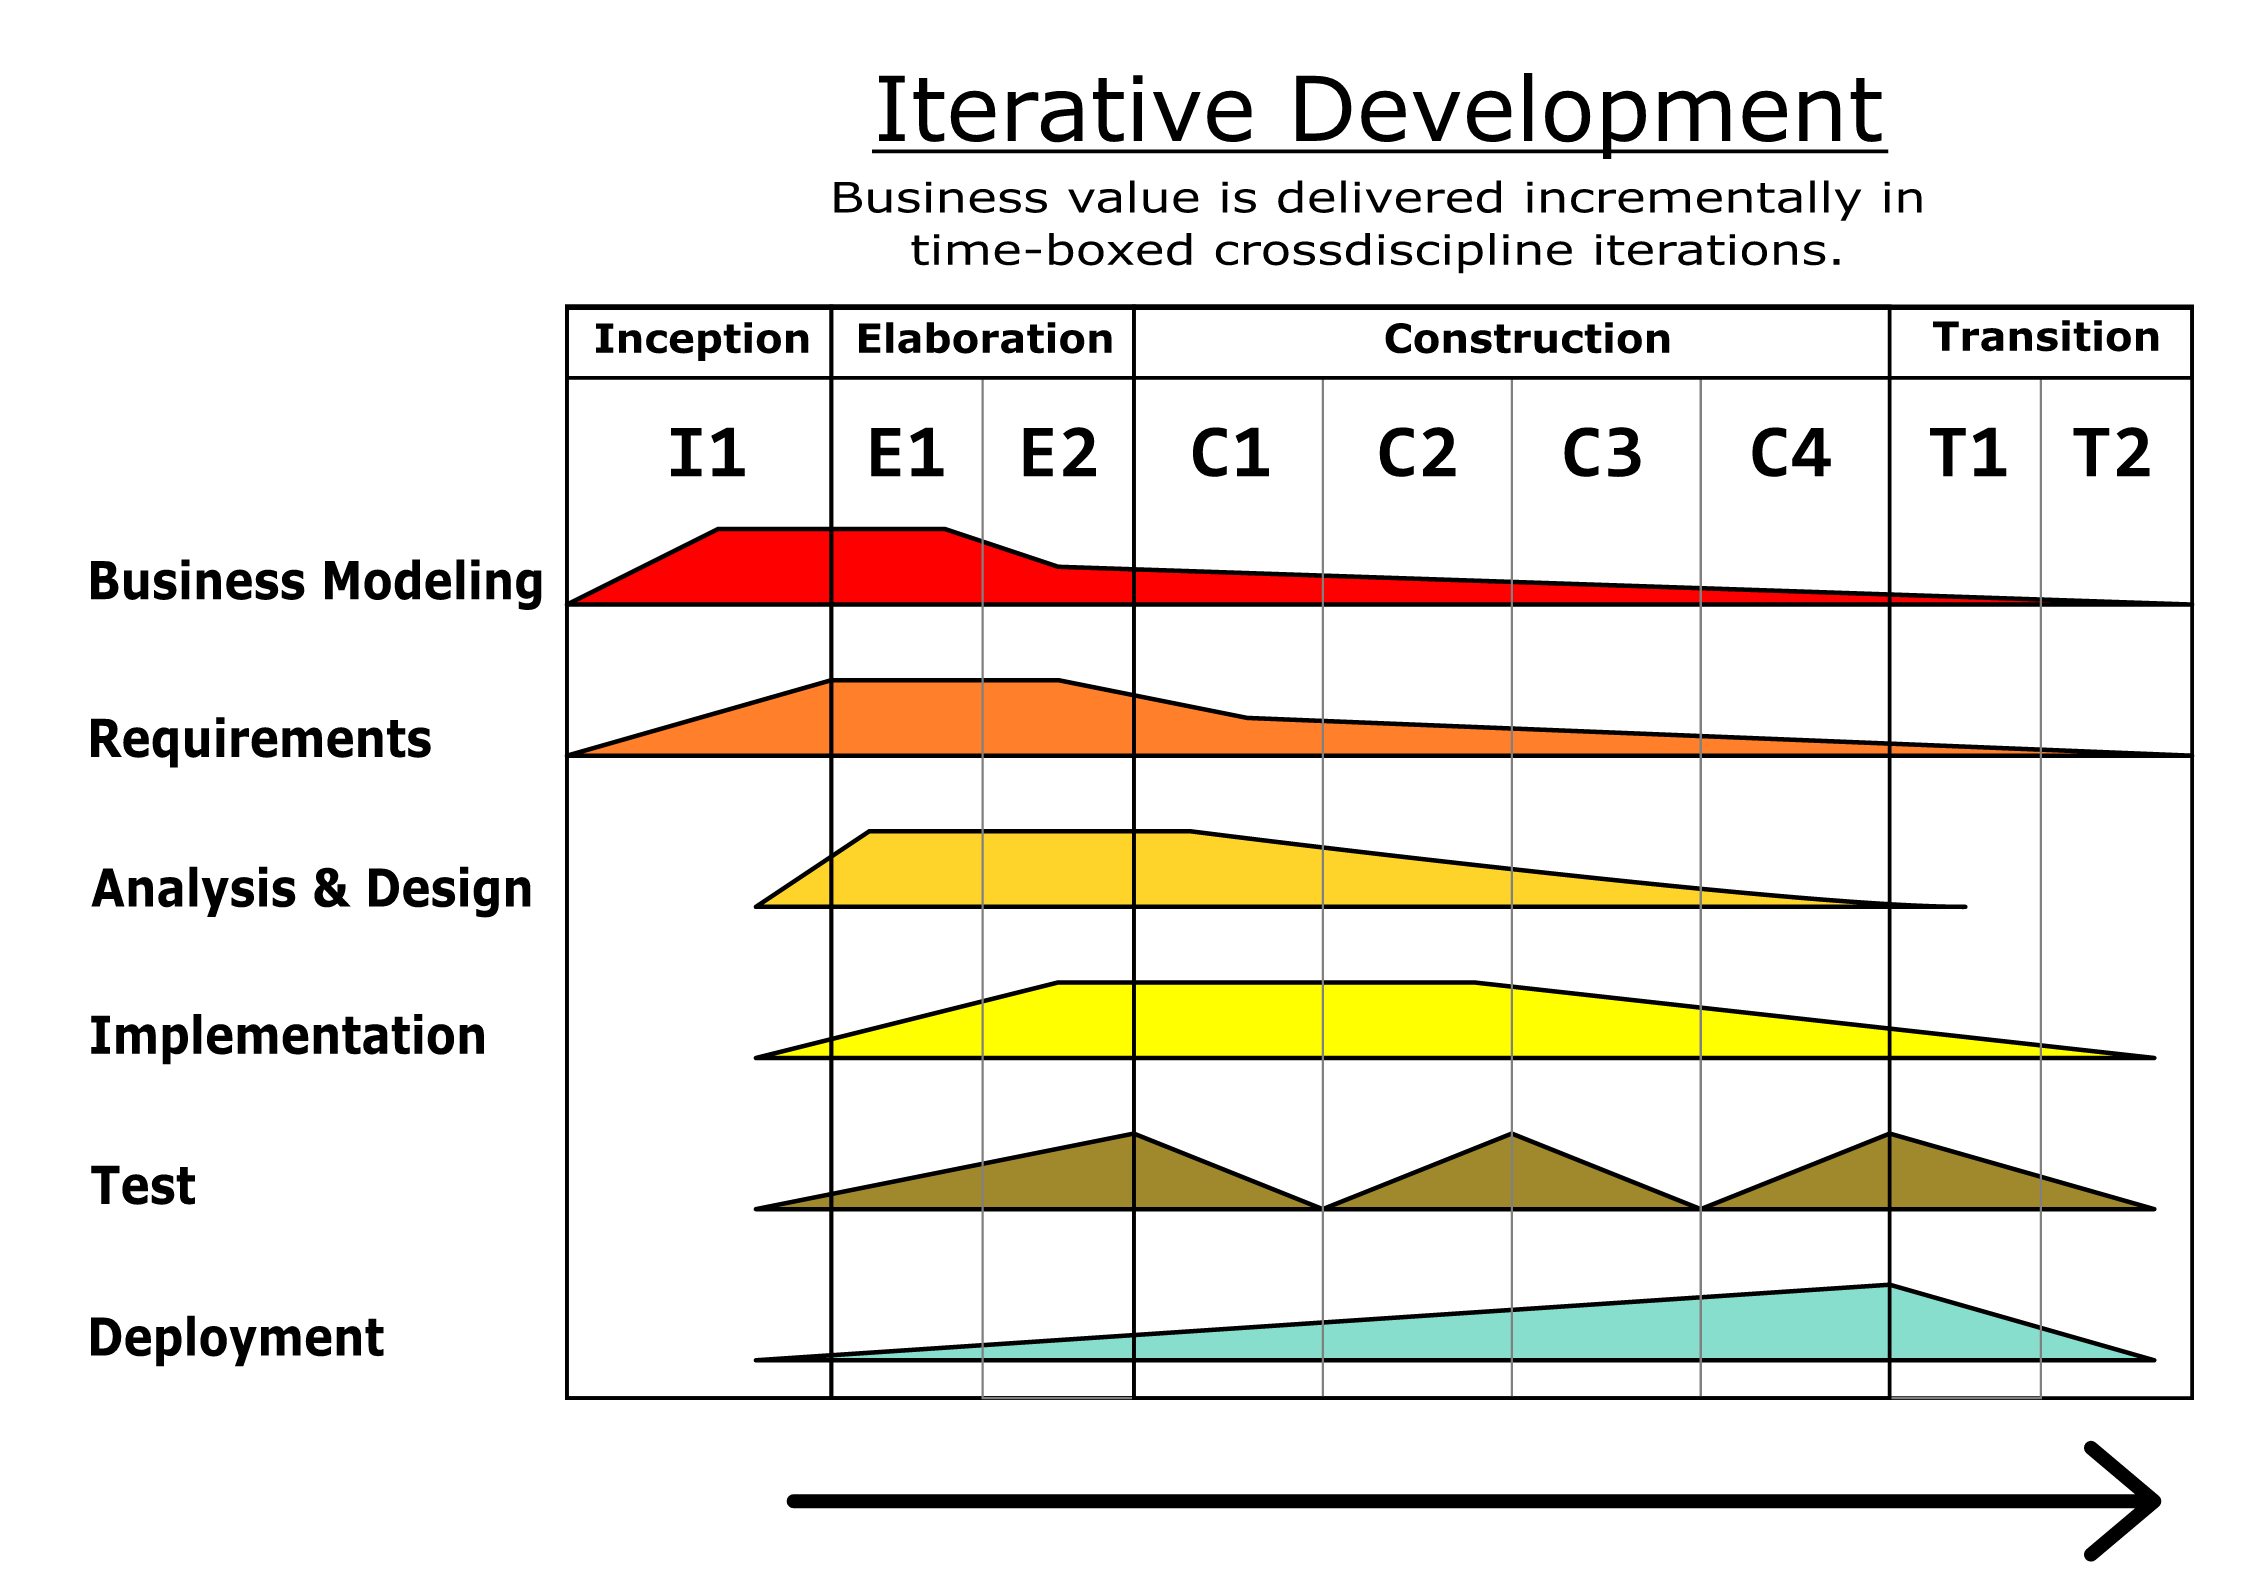
\includegraphics[width=0.9\textwidth,max height=0.58\textheight,keepaspectratio]{artifacts/unified-process-model.png}
  \caption{Unified Process-style lifecycle model showing time boxes and the change of focus over time.}
  \label{fig:unified-process}
\end{figure}

Figure~\ref{fig:unified-process} shows a Unified Process-style lifecycle model applied to the project's software development lifecycle. The model organized recurring disciplines such as requirements, design, implementation, validation, and documentation. The sprint workflow turned those disciplines into short implementation increments with concrete deliverables.

\begin{table}[H]
\centering
\begin{tabularx}{\textwidth}{P{0.20\textwidth}YY}
\toprule
\textbf{Method element} & \textbf{Use in the project} & \textbf{Reason} \\
\midrule
Unified Process-style lifecycle & Used as an overall SDLC planning model with overlapping disciplines. & Requirements, design, implementation, and validation had to evolve together. \\
Sprint workflow & Used to divide the work into short increments. & The prototype needed frequent integration and adjustment as technical risks became visible. \\
Risk-driven development & High-risk workflow boundaries were implemented early. & Capture, extraction, validation, review, and submission had to work together. \\
\bottomrule
\end{tabularx}
\caption{Methodological approach used in the project.}
\label{tab:method-approach}
\end{table}

Table~\ref{tab:method-approach} summarizes the methodological elements and why they were chosen. In this thesis, Unified Process-style (Table~\ref{tab:glossary}) means an iterative process where requirements, design, implementation, and testing overlap rather than run as one-way handovers.

\section{Project Phases}

The work was divided into five practical phases. The phases were not strict handover points. Later implementation work still affected requirements and design, but the phase structure made the work easier to plan, implement, and document. Table~\ref{tab:project-phases} lists the phase outputs.

\begin{table}[H]
\centering
\begin{tabularx}{\textwidth}{P{0.15\textwidth}YYY}
\toprule
\textbf{Phase} & \textbf{Main question} & \textbf{Work performed} & \textbf{Output} \\
\midrule
Discovery & What problem should the prototype solve? & Analysed the project brief, meeting notes, label fields, and workflow constraints. & Scope, field list, initial requirements. \\
Foundation & Can the app support the basic workflow? & Created Expo project structure, routing, local storage, and capture/import flow. & Running app skeleton with persisted attempts. \\
Extraction & Can label evidence become structured data? & Added barcode detection, provider-based vision-language extraction, prompt contract, parsing, and schema validation. & Draft AI-generated structured JSON from label images. \\
Review and ingest & Can the user safely accept and send data? & Added Confirm and Edit screen, accepted payloads, HTTP submission, idempotency, and offline queue. & Reviewed payload submission flow. \\
Hardening & Is the prototype reliable enough to demonstrate? & Added settings, diagnostics, retry behavior, automated tests, and documentation. & Testable prototype and thesis evidence. \\
\bottomrule
\end{tabularx}
\caption{Project phases and outputs.}
\label{tab:project-phases}
\end{table}

\section{Requirements Elicitation and Refinement}

Requirements were collected from the external project brief, the Buy2Sell meeting, and implementation findings. The requirements were then organized into functional requirements, non-functional requirements, and KPI targets, as shown in Table~\ref{tab:requirement-sources}.

\begin{table}[H]
\centering
\begin{tabularx}{\textwidth}{P{0.19\textwidth}YY}
\toprule
\textbf{Source} & \textbf{Input} & \textbf{Resulting requirements} \\
\midrule
Project brief & Manual registration, OCR and barcode idea, manufacturer and model extraction. & Capture, barcode decoding, structured extraction, registration payload. \\
Buy2Sell meeting & Multiple images, remote processing first, simulated server, previous-value suggestions, answerable fields only. & Multi-image requirement, configurable ingest endpoint, review step, field filtering. \\
Implementation findings & Provider output may be malformed, network delivery may fail, browser barcode support varies. & Schema validation, retry handling, offline queue, diagnostics, fallback behavior. \\
\bottomrule
\end{tabularx}
\caption{Requirement sources and their effect on the prototype.}
\label{tab:requirement-sources}
\end{table}

\section{Key Engineering Decisions}

Several decisions were made during development because of project constraints, technology constraints, and workflow risks.

\begin{table}[H]
\centering
\begin{tabularx}{\textwidth}{P{0.20\textwidth}P{0.23\textwidth}YP{0.18\textwidth}}
\toprule
\textbf{Decision} & \textbf{Alternatives considered} & \textbf{Reason} & \textbf{Consequence} \\
\midrule
Use Expo managed workflow & Bare React Native, custom native modules. & Faster cross-platform development and access to camera, image picker, SQLite, and secure storage. & Local VLM execution was excluded from the prototype. \\
Use VLM-first extraction & OCR-only pipeline, OCR plus rules, OCR plus LLM. & The system needed field mapping, not only text transcription. & Provider output had to be validated and reviewed. \\
Keep barcode decoding separate & Let the VLM read barcodes from the image. & Barcode values are deterministic evidence when decoded successfully. & Barcodes are merged conservatively into the result. \\
Require human confirmation & Fully automatic submission. & Some fields are ambiguous or require operator judgement. & Submission only happens after user acceptance. \\
Use local queueing & Cancel submission on network error. & Workshop network and endpoint availability may vary. & Accepted payloads can be replayed later. \\
\bottomrule
\end{tabularx}
\caption{Key engineering decisions and consequences.}
\label{tab:key-decisions}
\end{table}

In Table~\ref{tab:key-decisions}, deterministic merge means that extracted values are combined using fixed rules: barcode evidence is deduplicated, preserved in enrichment fields, and used to suggest \path{eanOrUpc} only for compatible barcode types. Ambiguous barcode candidates are recorded as conflicts instead of silently overwriting structured fields.

\section{Development Workflow}

The development workflow followed the primary application loop. Each increment extended or hardened the path from image capture to reviewed payload submission.

\begin{table}[H]
\centering
\begin{tabularx}{\textwidth}{P{0.19\textwidth}YY}
\toprule
\textbf{Increment} & \textbf{Goal} & \textbf{Validation} \\
\midrule
Capture/import & Create attempts from camera or gallery images. & Manual test and capture pipeline tests. \\
Extraction & Produce structured JSON from image evidence. & Provider parser tests, retry tests, schema validation tests. \\
Barcode enrichment & Detect and merge barcode evidence. & Barcode detector tests and merge tests. \\
Review & Let the user inspect and edit draft data. & Manual acceptance test and component tests. \\
Submission & Send accepted payloads to an endpoint. & Ingest transport and submission service tests. \\
Offline queue & Preserve accepted payloads when delivery fails. & Queue repository and queue worker tests. \\
Settings & Configure providers, endpoint, and credentials. & Settings repository and provider catalog tests. \\
\bottomrule
\end{tabularx}
\caption{Development increments and validation methods.}
\label{tab:development-increments}
\end{table}

\section{Technology Selection}
\label{sec:technology-selection}

Technology choices were made according to the prototype goals: cross-platform mobile support, camera access, local persistence, configurable remote extraction, and a reviewable JSON submission flow.

\begin{table}[H]
\centering
\begin{tabularx}{\textwidth}{P{0.20\textwidth}P{0.28\textwidth}Y}
\toprule
\textbf{Area} & \textbf{Selected technology} & \textbf{Reason} \\
\midrule
Mobile runtime & Expo and React Native & Cross-platform mobile implementation with web support and managed access to device features. \\
Routing & Expo Router & File-based navigation that matched the application screens. \\
Language & TypeScript & Static checking for structured data and service boundaries. \\
Persistence & Expo SQLite and Drizzle ORM & Local storage for attempts, settings, queue items, and typed database access through an ORM layer. \\
Validation & Zod & Runtime validation of model output and internal payloads. \\
AI integration & AI SDK provider adapters & Common abstraction for provider-based vision-language extraction. \\
Testing & Jest and React Native Testing Library & Automated validation of services, repositories, utilities, and selected UI behavior. \\
\bottomrule
\end{tabularx}
\caption{Technology choices and rationale.}
\label{tab:technology-selection}
\end{table}

Table~\ref{tab:technology-selection} also reflects a key tradeoff: Expo managed workflow supports portability and fast development, but it makes custom native model runtimes difficult. For that reason, local vision-language inference was treated as future work rather than part of the prototype.

Drizzle ORM (Table~\ref{tab:glossary}) was selected to keep SQLite access typed and centralized in repository code, instead of spreading handwritten SQL across screens and services.

\section{Validation Strategy}

Validation was divided into implementation validation, acceptance validation, and KPI evaluation.

\begin{table}[H]
\centering
\begin{tabularx}{\textwidth}{P{0.23\textwidth}YY}
\toprule
\textbf{Validation level} & \textbf{Purpose} & \textbf{Evidence} \\
\midrule
Implementation validation & Check technical behavior of services, repositories, schemas, retries, and queueing. & Automated Jest tests, type checking, linting. \\
Acceptance validation & Check that the operator can complete the capture-review-send workflow. & Manual end-to-end walkthroughs. \\
KPI evaluation & Measure extraction accuracy and define separate timing targets. & Extraction accuracy requires a fixed label dataset and reviewed ground truth. Time reduction requires a separate timed operator comparison. \\
\bottomrule
\end{tabularx}
\caption{Validation levels used in the project.}
\label{tab:validation-levels}
\end{table}

Automated tests validate the implemented workflow under expected and failure conditions. Extraction accuracy is handled separately in Chapter~\ref{chap:validation} because it requires real label images, reviewed ground truth, and semantic comparison. Registration time reduction is also separate because it depends on operator behavior, correction speed, and manual-entry baseline measurements.

\section{Method Limitations}

The methodology was suitable for building a working software prototype, but it does not by itself prove production effect. The project validates technical feasibility: image capture, barcode enrichment, provider-based extraction, schema validation, human review, submission, and offline queueing. Full business validation still requires timed manual baselines, production-build measurements, and evaluation inside the production registration workflow.
